\subsection{Consistency of local Voronoi diagrams}
\label{sec:localVoronoi}

In this section, we prove that the Voronoi diagram computed by the vehicle with a given lidar scan is consistent with the global Voronoi diagram computed from the map.
%
Intuitively, this proof formalizes the notion that a lidar with a sufficiently long range can detect all the edges for computing the Voronoi diagram for a small neighborhood.
%
The proof will formalize the requirements on the track and the range of the lidar.
%
At each point in time, only a subset of the walls are \emph{visible} to the lidar, i.e. all the walls in its range that are not occluded.
%
A \emph{local Voronoi diagram} is the Voronoi diagram of the visible walls.
%
The \emph{global Voronoi diagram} is the Voronoi diagram of all walls.
%
The planner chooses the waypoint from the intersection of the local Voronoi diagram and the lookahead circle.
%
Recall that the \emph{lookahead circle} is a circle of fixed radius centered at the rear axle of the car.
%
We also assume that the lidar is placed at the middle of the front axle of the car.
%
We give sufficient conditions such that within the lookahead circle the local and global Voronoi diagrams coincide.
%
% These conditions can be weakened, however it will complicate the proof so we refrain from it here.

Consider the visible subset of the walls, the local Voronoi diagram, and the lookahead circle at some arbitrary time.
%
Pick a point $p$ on the global Voronoi diagram inside the lookahead circle.
%
We give sufficient conditions such that the closest wall points to $p$ in the global Voronoi diagram are visible to the lidar. 
%
Thus, $p$ is also on the local Voronoi diagram.
%
The sufficient conditions rule out the two possible cases for invisibility of the closest wall points: being out of range, or occluded by a visible point.

Let $R$ be the range of lidar, 
$L$ the distance from lidar to the rear axle,
$\ell$ the lookahead radius,
$m$ the minimum width of the track,
$M$ the maximum width of the track,
and $D$ the minimum distance between lidar and the walls at any point in time.
Then we have the following guarantee:

\begin{theorem}
The local and global Voronoi diagrams coincide within the lookahead circle if
\begin{align}
    R > M, \\
    R > L + \ell + \frac{M}{2}, \label{eq:lidar-range-b} \\
    \textnormal{and,  } D^2 \geq (L+\ell)^2-\frac{m^2}{4}.\label{eq:lidar-wall-distance}
\end{align}
\label{thm:voronoi}
\end{theorem}

Before proving Theorem~\ref{thm:voronoi}, we will prove a lemma about the relationship between lookahead circle, walls of the circuit, and distance between a point on the Voronoi diagram and the walls.

\begin{lemma}
\begin{enumerate}
\item Any point on (local or global) Voronoi diagrams is at most $\frac{M}{2}$ away from its closest walls.
\item Lookahead disk is contained in the circle $C_{L+\ell}$ of radius $L+\ell$ centered at lidar.
\item For any point $p$ on the global Voronoi diagram inside $C_{L+\ell}$, $p$'s closest walls are in lidar's range.
\end{enumerate}
\end{lemma}
\begin{proof}
\begin{enumerate}
    \item 
    Lidar can see its closest walls since $R>M$. Furthermore, a point on the Voronoi diagram is equidistant to its closest walls.
    \item
    The distance from lidar to rear axle is $L$, and lookahead circle is the circle of radius $\ell$ centered at the rear axle.
    \item
    The closest wall points to $p$ are in the circle of radius $L+\ell+\frac{M}{2}$ centered at lidar. By Equation \ref{eq:lidar-range-b}, $p$'s closest wall points are in lidar's range.
\end{enumerate}
\end{proof}

\begin{proof}[Proof of Theorem \ref{thm:voronoi}]
We need to show that for any point $p$ on the global Voronoi diagram, if $p$ is inside the lookahead circle then $p$'s closest walls are visible from lidar, so that $p$ is also on the local Voronoi diagram.
%
By the lemma, the circle $C_{L+\ell}$ of radius $L+\ell$ centered at lidar contains the lookahead circle, so it is sufficient to assume that $p$ is in $C_{L+\ell}$.
Consider an arbitrary visible wall point $w$ occluding a wall point $u$.
That is, both $w$ and $u$ are on the same ray from lidar but $u$ is further away than $w$.
We show that $p$ is closer to $w$ than $u$.
Let $d$ be the distance of lidar to $w$ and $c$ be the distance of $w$ to $u$ (so the distance of lidar to $u$ is $d+c$).
First note that there is no Voronoi point inside the circle $C_{u, \frac{m}{2}}$ of radius $\frac{m}{2}$ centered at $u$, since $m$ is the minimum width of the track.
Also, the points that are closer to $u$ than $w$ constitute a half-plane $H$ with distance $d+\frac{c}{2}$ from lidar and its boundary being the bisector of $u$ and $w$.
Hence Voronoi points that are closer to $u$ than $w$ are in $H\setminus C_{u, \frac{m}{2}}$ i.e. in $H$ and outside of $C_{u, \frac{m}{2}}$.
See Fig. \ref{fig:voronoi-proof}.
If
$(d+\frac{c}{2})^2 + \frac{m^2}{4} - \frac{c^2}{4} > (L+\ell)^2$
or equivalently
$ d^2+dc > (L+\ell)^2-\frac{m^2}{4} $
then $C_{L+\ell}$ does not intersect $H\setminus C_{u, \frac{m}{2}}$.
The stronger condition 
\begin{equation}
     d^2 \geq (L+\ell)^2-\frac{m^2}{4}
\end{equation}
ensures that a global Voronoi point inside $C_{L+\ell}$ is closer to $w$ than any wall point in $w$'s shadow.
This inequality is guaranteed by Inequality \ref{eq:lidar-wall-distance}, since $D$ is the minimum distance of lidar to walls so $d^2 \geq D^2$.
\end{proof}

Observe that Theorem~\ref{thm:voronoi} gives us some bounds on the size of the lookahead circle. 
%
The lookahead circle cannot be too large, else, the closest walls to a points in the lookahead circle might be occluded from the lidar.

% \begin{figure}
% \centering
% 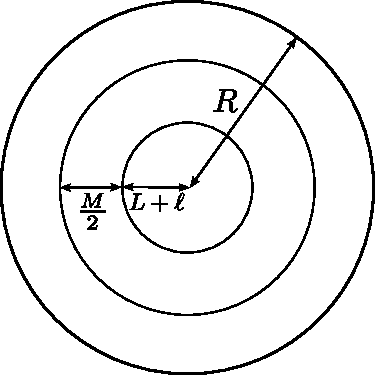
\includegraphics[width=1.5in]{Figures/voronoi-proof-a.pdf}
% \caption{Consistency of local and global Voronoi diagrams.}
% \label{fig:voronoi-proof-a}
% \end{figure}

\begin{figure}
\centering
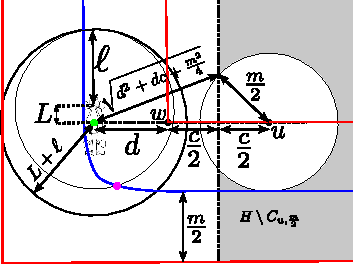
\includegraphics[width=2.5in]{Figures/voronoi-proof-shadow-distant.pdf}
\caption{Consistency of local and global Voronoi diagrams. The blue curve is the global Voronoi diagram. The green dot is lidar, and the pink dot is the waypoint. The gray area is $H\setminus C_{u, \frac{m}{2}}$. }
\label{fig:voronoi-proof}
\end{figure}




% Suppose a set of $n$ line segments
% $S = \{s_1, s_2, \ldots, s_n\}$
% in the Euclidean plane is given,
% where the line segments are pairwise disjoint except possibly at endpoints.
% The Voronoi Diagram $V(S)$ partitions the plane into Voronoi regions called as \emph{cells}.
% For each Voronoi cell $C$, there is a unique input line segment $s \in S$ such that
% all points in $C$ are closer to $s$ than to any line segment in $S - \{s\}$.
% A cell is defined using its boundary \emph{edges}.
% The edges may be linear or parabolic arcs.
% We illustrate the VD for line segments with a simple example. The reader can refer to ~\cite{Gold1995VoronoiDO} for more details.

% \textit{Example 1}.
% For given two 2-dimensional line segments,
% $\overline{ab}$ and $\overline{cd}$,
% their Voronoi edges are shown in blue in Fig.~\ref{fig:vd_segments}.
% The VD consists of two cells, $P$ and $Q$,
% where both are open. 
% The edges $\overline{uv}$, $\overline{wx}$ and $\overline{yz}$ are linear while $\overline{uw}$ and $\overline{xy}$ are parabolic.
% The Voronoi edges $\overline{yz}$ and $\overline{uv}$ are infinite. 

% \textbf{Remark}:
% Voronoi implementation in Boost generates two types of edges - \textit{primary} and \textit{secondary}. The edges highlighted in blue in Fig~\ref{fig:vd_segments} are primary because only primary edges are relevant to our work.
% ~\cite{voronoiboost} provides a detailed overview of the difference between primary and secondary edges.

% \begin{figure}[!t]
% \centering
% 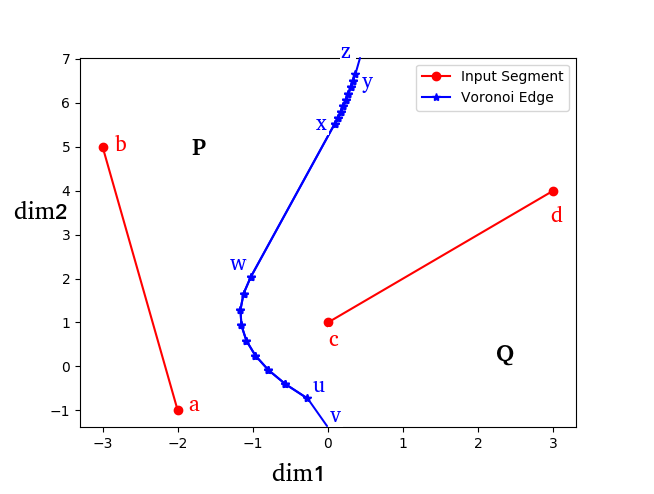
\includegraphics[width=3.45in]{Figures/voronoilabeled.png}
% \caption{Voronoi diagram: For line segments $\overline{ab}$ and $\overline{cd}$, their Voronoi diagram consists of two cells, $P$ and $Q$.}
% \label{fig:vd_segments}
% \end{figure}

% \begin{figure}[!t]
% \centering
% 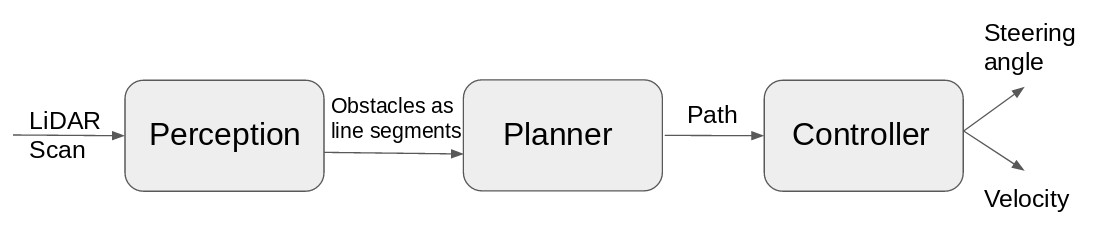
\includegraphics[width=3.4in]{Figures/block_diagram_voronoi.png}
% \caption{The problem addressed is given the sensor data, generate plan and obtain the control inputs - steering angle and velocity.}
% \label{fig:problem}
% \end{figure}